\chapter{\attekintes}

\section{Funkcionális áttekintés}

Munkám célja hogy mutasson egy olyan megközelítést, amelynek segítségével lehetséges gráfmintaillesztő
rendszerek tesztelése több aspektusból. Ezt úgy viszem véghez, hogy a rendszer nyelvén generálok
mintákat/lekérdezéseket, amelyeket aztán a lekérdező motoron futtatok. A generálásnak az az előnye,
hogy sok és diverz lekérdezést lehet így elkészíteni, ezért a nagy lekérdezéshalmaz alkalmassá válik
arra hogy teljesítményben tesztelje a lekérdező rendszereket. Illetve ha egyes lekérdezéseken nem tud
futtatni a rendszer akkor kiderül az is hogy milyen funkcionalitásokat nem fed még le. Egy 
referencia implementáció segítségével azt is ellenőrizni tudjuk, hogy a megfelelő válaszokat adja-e
a rendszer, hibás-e a működése. A megközelítésemet egy Neo4J \cite{neo4j} gráf adatbázison mutatom be 
miközben a lekérdezéseket az ehhez kifejlesztet Cypher \cite{Cypher} nyelven generálom.

Az elképzelést \aref{fig:funkcionalisAttekintes} ábrán mutatom be. A \textbf{Nyelvi specifikációt} a slizaa \cite{slizaa_2018} által készített openCypher EMF \cite{EMF} metamodell felhasználásával készítettem el. Az ott található metamodellt leszűkítettem a
cypher nyelvű \mm{SinglePartQuery} lekérdezések metamodelljére. Az \textbf{esettanulmány szignatúráját} a trainbenchmark \cite{szarnyas2018train} által használt szignatúra felhasználásával készítettem el. A \textbf{lekérdezés generátort} bővebben a következő szekcióban mutatom be. A \textbf{generált lekérdezéseket} egyaránt 

\begin{figure}
	\centering
	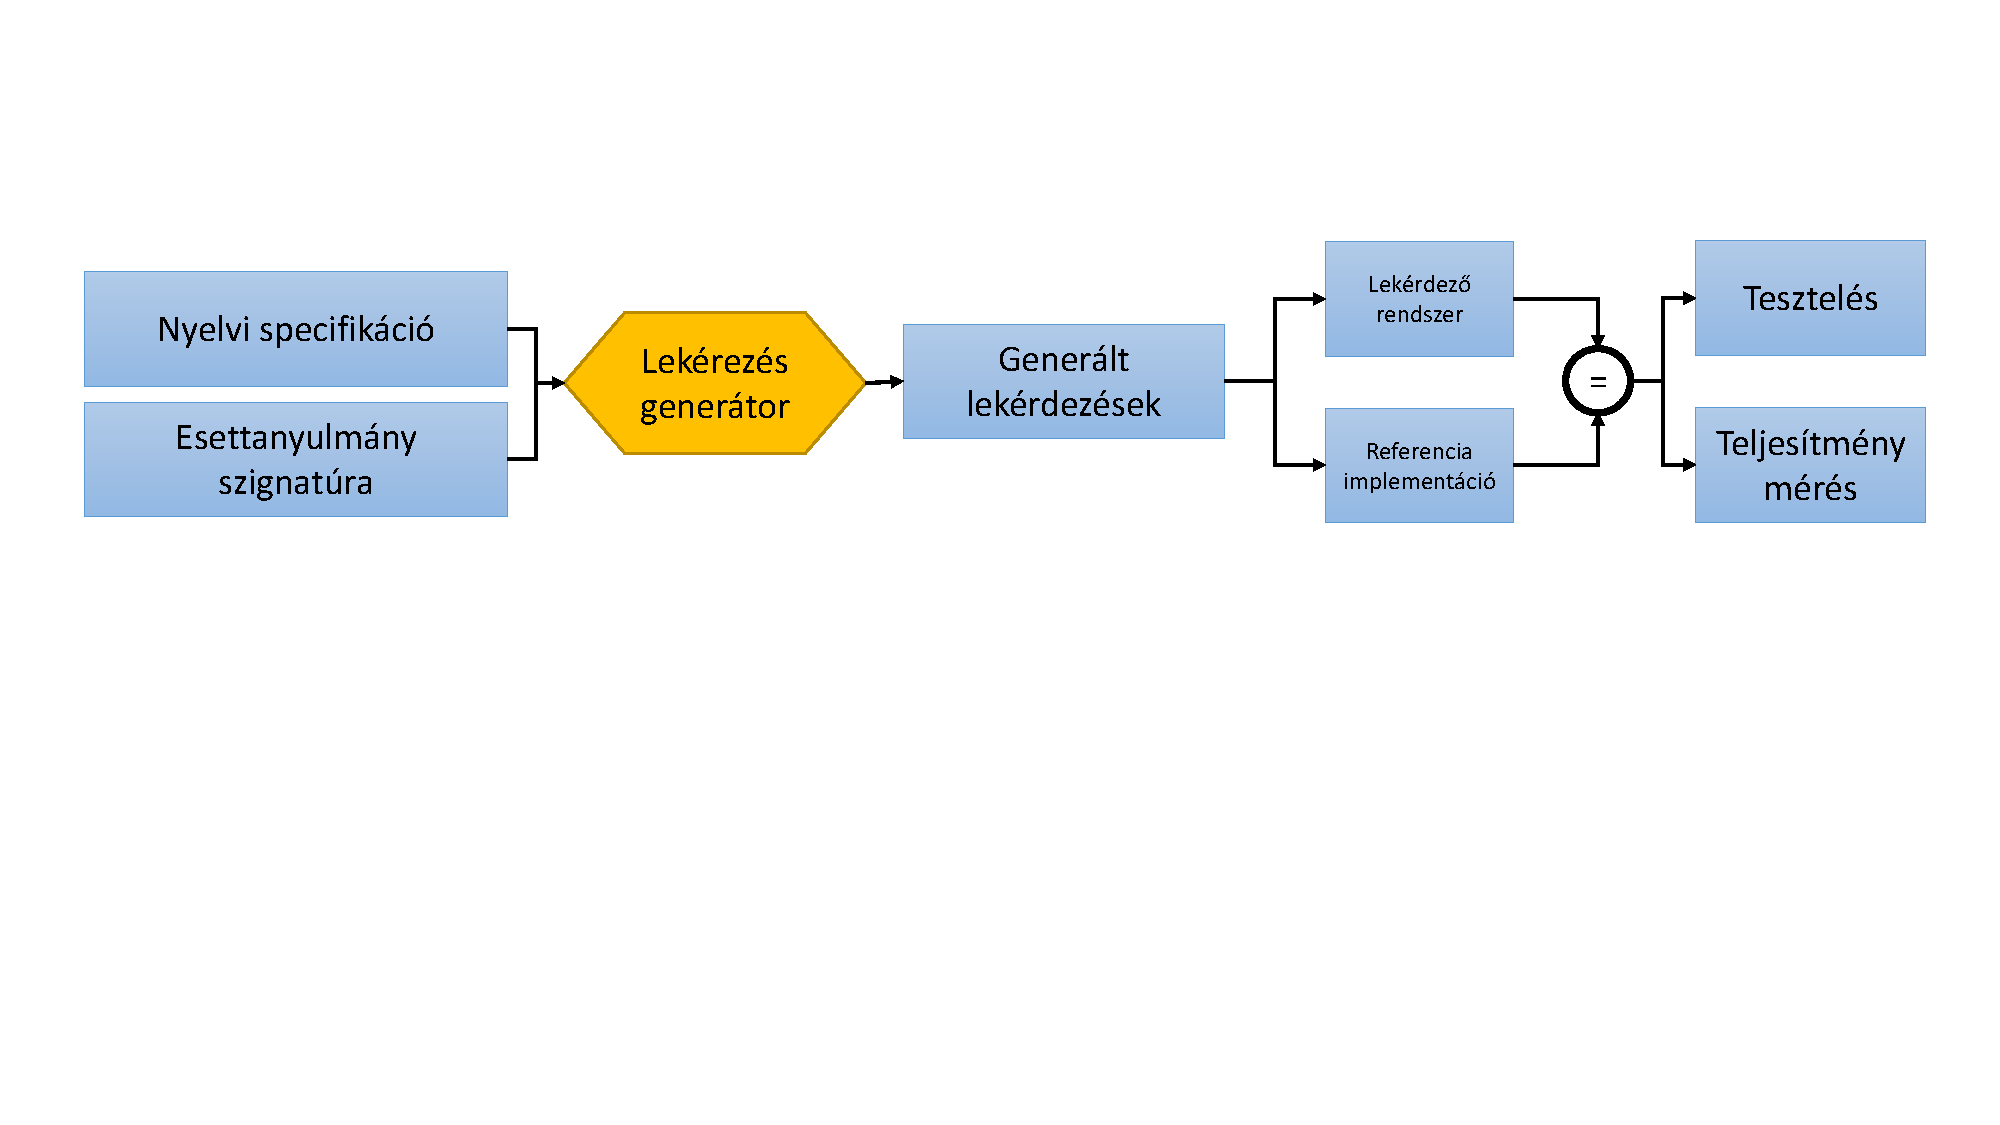
\includegraphics[width=0.7\textwidth]{figures/funkcionalisAttekintes}
	\caption{Az elképzelés funkcionális áttekintése}
	\label{fig:funkcionalisAttekintes}
\end{figure}
 
 

 
A generálást gráfok segítségével végzem,  a Viatra Solver keretrendszer felhasználásával. Ehhez első lépésben
szükség van a nyelv specifikációjának formális megadására
\begin{itemize}
	\item \textbf{Metamodell:} 
	\item \textbf{Metamodell:} 
	\item \textbf{Metamodell:} 
	\item \textbf{Metamodell:} 
\end{itemize}


aminek alapján példánymodelleket tudok generálni az adott nyelv felépítését betartva. Azonban vannak 
olyan szabályok amelyeket a metamodell nem fejez ki, betartásuk nélkül viszont a generált példánygráfok
nem értelmezhetőek Cypher nyelvű lekérdezésekként. Ezen szabályok betartására jólformáltsági kényszereket 
írok fel, amelyeket a generátor támpontként használ a lekérdezések készítése során. Ahhoz hogy mindezt 
véghez tudjam vinni választanom kellett egy gráf generáló szoftvert ami kényszerek és egy metamodell
alapján képes hatékonyan példánymodellek generállására. Ehhez a ViatraSolver nevű alkalmazást választottam,
ami eclipse fejlesztői környezetben működik, a jólformálsági kényszereket pedig Viatra nyelven írtam fel.

Miután a példánygráfok létrejönnek már csak le kell őket fordítani Cypher nyelvű lekérdezésekre.
A fordítás során ki kell tölteni a gráfgenerátor által üresen hagyott értékeket. Illetve ki kell sorosítani a
gráfokat egy .cypher típusú fájlba.  
  

\section{Lekérdezés generálási folyamat felépítése}

